\chapter{Analyses}\label{ch:Analyses}
In this chapter, an analysis of the data collected via the methods described in
the previous chapter (Chapter~\ref{ch:Methods}) is given. Firstly, a brief
initial overview is provided, where descriptive statistics of the equilibria
obtained and the overall characteristics of the strategies used is discussed.
Following this, a critical analysis of the p-thresholds obtained is carried out.
Here, the environmental effects, on the outcome of the game, discussed include:
number and characteristics of opponents; noise; and degeneracy. Then a
large-scale multivariate analysis is executed before considering the reliability
of the collected data. Note, as of writing, the database currently has 
\input{../../../src/database-code/data/se/20_01_2020/entries-in-database.txt}
entries (rows) and a total number of 
\input{../../../src/database-code/data/se/20_01_2020/number-of-tournaments}
tournament sets. 

\section{Initial Analysis}\label{sec:Initial_Analysis}
In this section, all the data (including those games which could be degenerate)
are considered. Taking a brief look at the graphs produced for each game, it can
be seen that the main `shapes' obtained are as seen in
Figure~\ref{fig:example_graphs}.

\begin{figure}
    \centering
    \begin{subfigure}[0.3\textwidth]
        \centering
        \includegraphics[width=\textwidth]{folk_thm/single_game/2/0/0.0/main.pdf}
        \caption{An example of a graph with a clear p-threshold point of approximately 0.28. In this game there is no degeneracy and the opponent strategy playing in the tournament was \textit{Inverse}, without noise.}
    \end{subfigure}\label{subfig:clear_thresh_plot}
    \begin{subfigure}[0.3\textwidth]
        \centering
        \includegraphics[width=\textwidth]{folk_thm/single_game/6/110/0.0/main.pdf}
        \caption{An example of a graph where the p-threshold is not as clear. Perhaps this is due to a small amount of noise and hence not enough repetitions and / or stochasticity of the players. In this case the threshold seems to lie in the range [0.1, 0.3]. There is no degeneracy in this game and opponent strategies in the tournament were: \textit{Feld: 1.0, 0.5, 200}; \textit{Cooperator};  \textit{EvolvedLookerUp2_2_2}; \textit{Tullock: 11}; and \textit{ZD-GEN-2: 0.125, 0.5, 3}. Again, this tournament was run with no added noise.}
    \end{subfigure}\label{subfig:unclear_thresh_plot}
    \begin{subfigure}[0.3\textwidth]
        \centering
        \includegraphics[width=\textwidth]{folk_thm/single_game/5/77/0.0/main.pdf}
        \caption{An example of a graph where the p-threshold is not clear at all due to some (or all) of the games, which were played by the particular tournament set, being degenerate. In this case, the strategies playing in the tournament were: \textit{Random: 0.5}; \textit{Grumpy: Nice, 10, -10}; \textit{Fortress3}; and \textit{Negation}. This tournament had no added noise.}
    \end{subfigure}\label{subfig:degenerate_plot}
    \caption{Example graphs obtained from the experiment.}\label{fig:example_graphs}
\end{figure}

This will be discussed further in the next section as follows:
Figure~\ref{subfig:clear_thresh_plot}, and general properties of the
p-threshold, will be described in Section~\ref{sec:Analysis_of_the_p-Threshold};
the stochasticity and accuracy visible in
Figure~\ref{subfig:unclear_thresh_plot} will be analysed in
Sections~\ref{subfig:Effects_of_Stochastic_Players}
and~\ref{subsec:Accuracy_of_Thresholds}, respectively; and finally
Figure~\ref{subfig:degenerate_plot}, and degeneracy overall, will be considered
in Section~\ref{subsec:Effects_of_Degeneracy}.

\begin{figure}
    \centering
    \includegraphics[width=\textwidth]{folk_thm/initial_analysis/summary_stats.html
    }
    \caption{A table of the summary statistics produced from the data of the experiment.}\label{fig:summary_stats}
\end{figure}

The summary statistics gained from running the \textit{describe()} method of a
pandas database is given in Figure~\ref{fig:summary_stats}. From this, it can be
seen that the number of opponents the \textit{Defector} played against ranged
from one to seven, with an average of four opponents. Also, as expected, the
mean probability of the game ending encountered was 0.5. Observe that, overall,
there were 175,399 distinct tournaments played (\textit{experiment_number}) with
a total of 159 distinct sets of strategies (\textit{tournament_player_set}).
Looking now at the statistics for Nash equilibria, it can be seen that a total
of 823,823 equilibrium points were calculated in this experiment, with an
average of \(1.914 \approx 2\) equilibria per game. However, observe, at least
one game obtained 39 equilibria which will be explored into later on in this
section. Considering the probabilities of defection within these equilibria,
notice that both the greatest and the least probabilities of defection ranged
from zero to one inclusive with a \(50\)th percentile of zero. But, looking at
the average values, the least probability has a mean of 0.342 and only just
above this, the greatest probability has a mean of 0.460.

Next, further descriptive statistics are calculated for the strategies. This is
to obtain a more in-depth view on the types of strategies randomly chosen to
play and their characteristics. Executing \textit{value_counts()} method on the
column of strategy names, it is observed that the player which appeared the most
times (9 times) is \textit{ZD-GEN-2: 0.125, 0.5, 3}; followed closely by
\textit{Tideman and Chieruzzi} with 7 sets of tournaments. On the other hand 38
out of the 200 strategies playing in this experiment appeared only once.
Running the \textit{value_counts()} method again, but this time on the memory
depths of the strategies found the majority of strategies to have an infinite
memory depth. On the other hand, strategies having no memory or a depth equal to
one were significant. Considering the stochasticity of players alongside how
many appearances each strategy made yielded the following chart in
Figure~\ref{fig:stochastic_chart}.

\begin{figure}
    \centering
    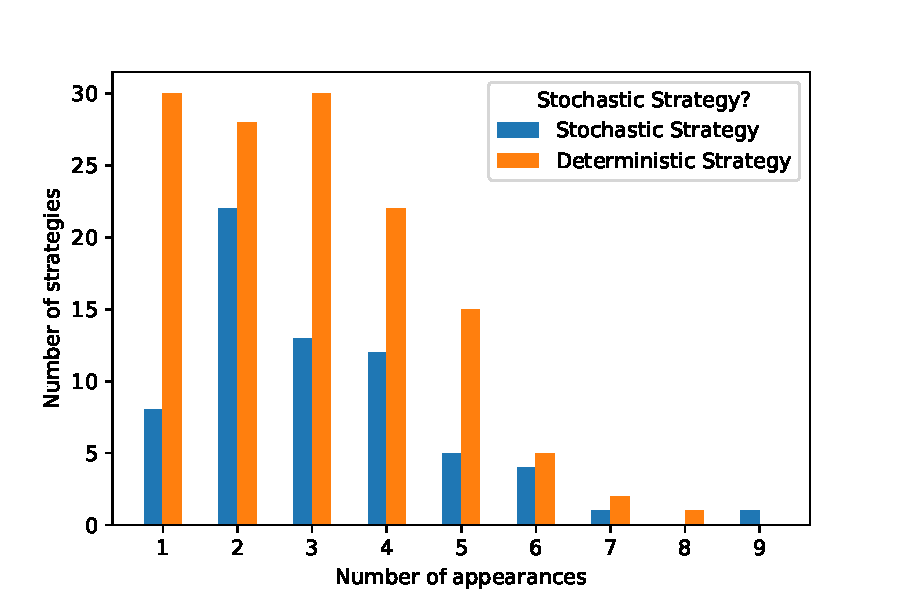
\includegraphics[width=\textwidth]{folk_thm/initial_analysis/strategy_appearances.pdf}
    \caption{A plot to show the ratio of stochastic to deterministic strategies randomly chosen throughout the experiment.}\label{fig:stochastic_chart}
\end{figure}

It is clear that there is a clear bias towards deterministic strategies
in this experiment. However, this is to be expected as running the following
code:
\begin{minted}[frame = lines, framesep = 2mm, fontsize = \scriptsize, bgcolor = Cornsilk]{python}
    len(axl.filtered_strategies(filterset={"stochastic": True})), 
    len(axl.filtered_strategies(filterset={"stochastic": False}))

    (86, 156)
\end{minted}
it can be seen that over half the strategies coded into the Axelrod library are
classed as deterministic. Looking at Figure~\ref{fig:stochastic_chart} again,
observe, the majority of deterministic strategies were executed either once or
three times. On the other hand, a large proportion of the stochastic strategies
were played twice.

Further, the number of Nash equilibria obtained for each game was analysed and
their distributions with respect to the number of opponents of the
\textit{Defector} plotted. Executing the \textit{value counts} method on the
`num_of_equilibria' column gave the following conclusions: 

\section{Analysis of the p-Threshold}\label{sec:Analysis_of_the_p-Threshold}
Firstly, two csv files were obtained from the 
\subsection{Effects of the Number of Players}\label{subsec:Effects_of_the_number_of_Players}

\subsection{Effects of Stochastic Players}\label{subsec:Effects_of_Stochastic_Players}

\subsection{Effects of Noise}\label{subsec:Effects_of_Noise}

\subsection{Effects of Degeneracy}\label{subsec:Effects_of_Degeneracy}

\section{Multivariate Data Analysis}\label{sec:MV_Data_Analysis}

\section{Reliability of Data}\label{sec:Reliability_of_Data}

\subsection{Comparison of Databases}\label{subsec:Comparison_of_Databases}

\subsection{Accuracy of Thresholds}\label{subsec:Accuracy_of_Thresholds}